
\chapter{Classification}
\label{ch:capitolo3}
Classification was performed on the available training set using three different algorithms: K-NN (\textit{K-Nearest Neighbours}), Naïve Bayes and Decision Trees.
For K-NN \textbf{and Naïve Bayes}, a portion of the training set (referred to as the validation set) was used to select the best hyperparameters \textbf{each} model.
The features used in K-NN and Naïve Bayes were normalized, as these models are sensitive to unscaled values.
In particular, a log-transformation and \textbf{SCRIVERE SE StandardScaler O MINMAX} were applied to data.
After training, the models were evaluated on the test set using standard performance metrics. 
The target variables chosen for this task are 2: \texttt{titleType}, and \texttt{has\_LowEngagement}.
These will be discussed in more detail in the corresponding sections below.

\section{Binary classification}\label{sec:binary_classification}
The binary target variable used in this task, \texttt{has\_LowEngagement}, was specifically defined for this purpose. 
It identifies records where the \texttt{numVotes} attribute is less than 100.
\subsection*{K-NN}


\subsection*{Naïve Bayes}


\subsection*{Decision Trees}
To identify the optimal hyperparameters for the Decision Tree model, a Randomized Search with
Cross-Validation was conducted on the training set.
The best configuration found used the Gini index as the splitting criterion,
a maximum tree depth of 26, and a minimum of 3 samples per leaf.
Post-pruning did not yield any performance improvement and was therefore not applied.
The classification performance of the final model is summarized in
Table~\ref{tab:binary_classification_report}.

\begin{table}[H]
    \centering
    \begin{tabular}{lcccc}
        \toprule
        \bf{Class} & \bf{Precision} & \bf{Recall} & \bf{F1-score} & \bf{Support} \\
        % \midrule
        % \bf{Train set} & & & & \\
        % \midrule
        % \bf{Low engagement} & 0.87 & 0.91 & 0.89 & 4668 \\
        % \bf{High engagement} & 0.78 & 0.70 & 0.74 & 10287 \\
        % \midrule
        % \bf{Test set} & & & & \\
        \midrule
        \bf{Low engagement} & 0.86 & 0.90 & 0.88 & 3416 \\
        \bf{High engagement} & 0.75 & 0.68 & 0.71 & 1561 \\
        \midrule
        \bf{Macro avg} & 0.80 & 0.79 & 0.80 & \\
        \bf{Weighted avg} & 0.83 & 0.83 & 0.83 & \\
        \midrule
        \bf{Accuracy}  &  &  & 0.83 & \\
        \bottomrule
    \end{tabular}
    \caption{Classification report for binary classification}
    \label{tab:binary_classification_report}
\end{table}


\begin{figure}[h]
    \begin{minipage}{0.58\textwidth}
        Figure~\ref{fig:conf_matr_binary_dt} shows the confusion matrix for the obtained
        Decision Tree, with results regarding the test set.
        As can be seen, a significant number of \textit{High Engagement} records was misclassified,
        leading to a low Recall.
        This might be a consequence of class imbalance, as well as the possible presence
        of noise in the data.
    \end{minipage}
    \hfill
    \begin{minipage}{0.38\textwidth}
        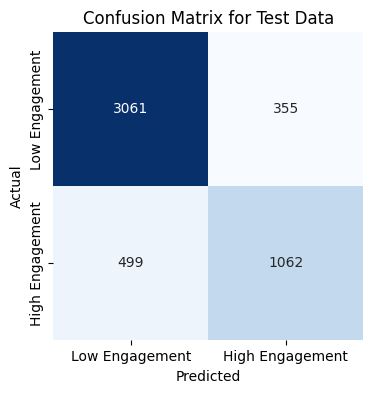
\includegraphics[width=\linewidth]{plots/binary_dt_confusion_matrix.png}
        \captionsetup{justification=centering, width=0.9\linewidth}
        \caption{Confusion matrix for binary classification}
        \label{fig:conf_matr_binary_dt}
    \end{minipage}
\end{figure}


\section{Multiclass classification}\label{sec:multiclass_classification}
Among the multiclass features of the training set, \texttt{titleType}
was chosen as the target variable for this task due to its relevance in the dataset.
Since \texttt{runtimeMinutes} main imputation method for missing values was done
with the aid of the target variable, to avoid data leakage, the feature was re-imputed
by simply sampling from the distribution of its values, without considering the \texttt{titleType}
feature.\\

% This feature was created to impute the missing values of the original \texttt{runtimeMinutes} variable,
% but without using the median value according to the titleType. Instead, the missing values were imputed using the help of two variables: \texttt{canHaveEpisodes} and \texttt{is\_Short}
% (as one of the resulting variables of the multi-label one-hot encoding process of the \texttt{genres} attribute).
% In particular, 
% \textbf{SCRIVERE COME E' STATA IMPUTATA NO\_TT - con canhaveepisodes e is\_short preso dai generi}.
% This approach prevents a significant error, as it would be methodologically incorrect to use \texttt{titleType}-based 
% imputation for an attribute when \texttt{titleType} itself is the target variable to predict.
\subsection*{K-NN}
\subsection*{Naïve Bayes}
\subsection*{Decision Trees}
\begin{table}[H]
    \centering
    \begin{tabular}{lcccc}
        \toprule
        \bf{Class} & \bf{Precision} & \bf{Recall} & \bf{F1-score} & \bf{Support} \\
        \midrule
        \bf{movie}         & 0.85 & 0.88 & 0.87 & 1877 \\
        \bf{short}         & 0.92 & 0.94 & 0.93 & 766 \\
        \bf{tvEpisode}     & 0.89 & 0.92 & 0.90 & 1599 \\
        \bf{tvMiniSeries}  & 0.51 & 0.35 & 0.41 & 81 \\
        \bf{tvMovie}       & 0.36 & 0.29 & 0.32 & 299 \\
        \bf{tvSeries}      & 0.89 & 0.94 & 0.91 & 447 \\
        \bf{tvShort}       & 0.00 & 0.00 & 0.00 & 16 \\
        \bf{tvSpecial}     & 0.32 & 0.12 & 0.18 & 49 \\
        \bf{video}         & 0.55 & 0.46 & 0.50 & 250 \\
        \midrule
        \bf{Macro avg}     & 0.59 & 0.54 & 0.56 & 5384 \\
        \bf{Weighted avg}  & 0.82 & 0.84 & 0.83 & 5384 \\
        \midrule
        \bf{Accuracy}      &      &      & 0.84 & 5384 \\
        \bottomrule
    \end{tabular}
    \caption{Classification report for multiclass classification (\texttt{titleType})}
    \label{tab:multiclass_classification_report}
\end{table}




\section{General considerations}\label{sec:general_considerations}
